\documentclass[11pt]{article}

% ---------------------------------------------------------------------
% Packages
% ---------------------------------------------------------------------
\usepackage[a4paper,margin=1in]{geometry}
\usepackage[T1]{fontenc}
\IfFileExists{lmodern.sty}{\usepackage{lmodern}}{\usepackage{mathptmx}}
\usepackage{microtype}
\usepackage{amsmath,amssymb,amsfonts,bm}
\usepackage{booktabs,tabularx,multirow,array}
\usepackage{graphicx}
\usepackage[dvipsnames]{xcolor}
\usepackage{tikz}
\usetikzlibrary{arrows.meta,positioning,fit,calc,shapes.geometric}
\usepackage[ruled,vlined,linesnumbered]{algorithm2e}
\usepackage{listings}
\usepackage{enumitem}
\usepackage[font=small,labelfont=bf]{caption}
\usepackage[numbers,sort&compress]{natbib}
\usepackage[colorlinks=true,linkcolor=MidnightBlue,citecolor=MidnightBlue,urlcolor=MidnightBlue]{hyperref}
\usepackage[capitalise,noabbrev]{cleveref}

% ---------------------------------------------------------------------
% Macros
% ---------------------------------------------------------------------
\newcommand{\Hst}{\mathcal{H}}           % hypothesis history
\newcommand{\Est}{\mathcal{E}}           % evidence log
\newcommand{\Mst}{\mathcal{M}}           % shared memory
\newcommand{\opp}{\mathcal{O}}           % opponent pool
\newcommand{\reg}{\mathcal{R}}           % metric registry
\newcommand{\E}{\mathbb{E}}
\newcommand{\KL}{D_{\mathrm{KL}}}
\newcommand{\gbar}{\bar{g}}
\newcommand{\code}[1]{\texttt{\small #1}}
\newcommand{\todo}[1]{\textcolor{BrickRed}{[\textbf{TODO:} #1]}}
\newcommand{\pUp}{\textsc{up}}
\newcommand{\pFlat}{\textsc{flat}}
\newcommand{\pDown}{\textsc{down}}

\lstdefinestyle{json}{
  basicstyle=\ttfamily\footnotesize,
  breaklines=true,
  frame=single,
  framerule=0.3pt,
  rulecolor=\color{gray!60},
  backgroundcolor=\color{gray!4},
  columns=fullflexible,
  keepspaces=true,
  showstringspaces=false
}

\title{\textbf{Coach LLM: Evidence-Grounded Refinement of Tactical Hypotheses\\for Multi-Agent Reinforcement Learning}}
\author{Baofeng Zhang\\[2pt]\small Nagoya University\\\small zhang.baofeng@g.sp.m.is.nagoya-u.ac.jp}
\date{\today}

\begin{document}
\maketitle

% =====================================================================
\begin{abstract}
Large language models (LLMs) are increasingly used to turn guidance in natural language into objectives for multi-agent reinforcement learning (MARL).
In existing pipelines the guidance itself is treated as fixed: an instruction is mapped once to a reward, a waypoint or a skill, or reward code is searched to maximize performance on a fixed task.
We study a different question: can an LLM \emph{coach} revise the tactical hypothesis itself in light of the behavioral evidence that MARL training produces?
We represent a tactic as a structured hypothesis $H=(C,A,M,O)$ of condition, action, mechanism and observable evidence, and let each hypothesis evolve along its own \emph{refinement chain}.
In every round the hypothesis is compiled through a typed domain-specific language (DSL) into a shaping potential with a soft gate, a frozen base policy is adapted against a fixed opponent pool, and the outcome is attributed through an execution--mediator--benefit decomposition that separates evidence about the tactic from engineering failures such as untriggered conditions or policies that did not move.
The Coach then revises the hypothesis with seven typed operators under constrained decoding, and every revision must still explain all earlier evidence on its chain.
After each round, a chain either continues to a next version or terminates, as a converged rule whose condition has been narrowed to its true range of applicability or as a retired hypothesis that the evidence has judged wrong.
Three append-only stores make every Coach prompt reproducible byte for byte, so that ablations of the Coach can be replayed on existing evidence at zero GPU cost.
We describe the framework, the design decisions forced by a budget of only tens of training runs, and an evaluation protocol on the MARLadona soccer environment.
\end{abstract}

% =====================================================================
\section{Introduction}
\label{sec:intro}

A soccer coach does not hand players a reward function.
A coach states a tactical idea, such as ``when the opponent is compact in the center, widen the shape'', watches what happens, and then revises the idea: perhaps it works only when the opponent's midfield is also high, or perhaps the gap it was supposed to open never appears.
The object being improved is the \emph{hypothesis}, not the policy that executes it.

Recent work connecting LLMs with (multi-agent) reinforcement learning has largely focused on the opposite direction.
LLMs write or select reward functions \citep{ma2024eureka,incentive2026,maestro2025}, rank states to learn dense potentials \citep{lin2025lca}, choose among a predefined pool of skill potentials \citep{ma2025vgepf}, emit subgoals or waypoints for low-level learners \citep{l2m2_2025,yano2025icco}, or produce structured commands that are grounded into reward shaping and action masks \citep{lehca2026}.
In all of these, the guidance expressed in language is an \emph{input}: it is either fixed by a human or optimized only insofar as it raises task return.
None asks whether the guidance was \emph{right}, under which conditions, and for which reason.

We frame this as \emph{evidence-grounded tactical belief refinement}.
A tactical hypothesis is written as $H=(C,A,M,O)$: a condition $C$ under which it applies, an action $A$ that our team should take, a mechanism $M$ explaining why it should work, and observable evidence $O$ that should appear in simulation if it does.
A Coach LLM proposes a version of $H$, the system compiles it into an executable objective, a MARL policy is adapted toward it, and the resulting behavior is turned into structured evidence.
The Coach then revises $H$, most often by narrowing $C$, and the loop repeats until the hypothesis converges or is retired.

Three properties of this setting make it substantially harder than the settings studied in recent work on LLM belief revision and AI scientists \citep{evoscm2026,labloop2026}:
\begin{itemize}[leftmargin=*,itemsep=2pt]
  \item \textbf{Expensive experiments.} One experiment is one MARL adaptation run, taking hours.
    A campaign affords on the order of tens of rounds, not thousands.
  \item \textbf{Noisy feedback with several possible causes.} A hypothesis may fail because the tactic is wrong, because its translation into an objective is wrong, because RL did not converge within budget, or because of seed noise.
    Only the first should change a belief.
  \item \textbf{No ground truth.} There is no unique correct causal model of soccer tactics to recover.
    The useful output is a rule with a clearly delimited range of applicability, not the identification of a true model.
\end{itemize}

\paragraph{Contributions.}
\begin{enumerate}[leftmargin=*,itemsep=2pt]
  \item A formulation of tactical guidance in MARL as \emph{condition refinement of a single hypothesis}, with refinement chains that end in an explicit terminal state (converged or retired) rather than an open-ended sequence of new hypotheses (\cref{sec:problem}).
  \item A decomposition of each outcome into three parts (\emph{execution}, \emph{mediator} and \emph{benefit}), together with two diagnostics (mean gate value and KL from the base policy) that programmatically separate evidence about the tactic from four kinds of engineering failure (\cref{sec:feedback}).
  \item A typed compilation path from hypotheses in coach language to shaping potentials with soft gates, whose output space is closed under constrained decoding and whose thresholds are expressed as percentiles of the base policy (\cref{sec:compile}).
  \item A Coach revision procedure with seven typed operators, preregistered directional predictions, and deductive validation by evidence replay, built on append-only stores that make every prompt reproducible byte for byte and every Coach ablation free of GPU cost (\cref{sec:revision,sec:stores}).
\end{enumerate}

\paragraph{Scope and status.}
We state the limitations of this draft up front.
(i) No empirical results are reported yet; \cref{sec:protocol} specifies the protocol and the analyses that will be run.
(ii) Several design parameters are still open, namely the global magnitude of the shaping term, the composition of the opponent pool, and whether MARLadona supports custom initial states; they and are flagged where they appear.
(iii) Efficiency figures in \cref{sec:efficiency} are estimates from general MARL experience, not measurements.

% =====================================================================
\section{Related Work}
\label{sec:related}

\paragraph{LLM-guided objectives for (multi-agent) RL.}
Eureka \citep{ma2024eureka} iteratively evolves reward code with an LLM, and \citet{incentive2026} extend this style of reward search to cooperative MARL with incentive diagnostics.
LCA \citep{lin2025lca} avoids direct reward writing by asking an LLM for preference judgments over agents' behavior and training a potential specific to each agent from these judgments; LaRe \citep{qu2025lare} uses an LLM to identify latent factors relevant to reward for temporal credit assignment.
V-GEPF \citep{ma2025vgepf} selects among a predefined pool of vision-language potentials to align MARL behavior with human instructions.
Hierarchical approaches use the LLM as a high-level policy emitting subgoals \citep{l2m2_2025} or as a commander whose structured output is grounded into reward shaping and action masks \citep{lehca2026}; ICCO \citep{yano2025icco} learns a coordinator that reconciles language instructions with the environment task.
MAESTRO \citep{maestro2025} lets an LLM shape the whole training process through curricula and templated reward parameters.
Across this line of work, the guidance is either fixed or optimized as a means to task return.
We borrow several mechanisms, namely structured JSON interfaces, potential-based shaping, and the idea that LLM judgments need not be raw reward code, but change the object of optimization from the policy's reward to the hypothesis itself.

\paragraph{LLM harnesses and self-improving agents.}
A large body of work improves a fixed LLM by engineering what surrounds it: interleaved reasoning and acting \citep{yao2023react}, verbal self-reflection stored in memory \citep{shinn2023reflexion}, critique grounded in tool use \citep{gou2024critic}, agent--computer interfaces \citep{yang2024sweagent}, grounding language in affordances \citep{ahn2022saycan}, delegating search to external planners \citep{liu2023llmp}, and memory, reflection and planning for long-horizon agents \citep{park2023generative}.
Other work optimizes the harness itself, from compiled prompt pipelines \citep{khattab2024dspy} to automatically designed agentic systems and workflows \citep{hu2025adas,zhang2025aflow}, skill libraries \citep{wang2023voyager}, and exploration policies tuned on replayed search histories \citep{dreamrsi2026}; see \citet{gao2026survey} for a survey.
Most of these methods improve \emph{procedural} knowledge, that is, how to reason or act.
Our Coach updates \emph{epistemic} content, that is, what is believed about the environment, and its harness is deliberately thin: a batch pipeline with structured stores rather than an agent framework.

\paragraph{LLM belief revision and AI scientists.}
EvoSCM \citep{evoscm2026} equips an LLM agent with an explicit population of structural causal models, designs discriminating interventions, and revises causal structure from prediction errors.
Work on lab-in-the-loop AI scientists \citep{labloop2026} maintains a structured hypothesis register with confidence and status labels and finds that genuine experimental feedback improves later performance while falsified feedback degrades it.
We share the commitment to explicit, falsifiable belief states and adopt the abduction--prediction / induction--revision structure, but our task differs in kind: we refine the applicability condition of a \emph{single} hypothesis rather than select a model from a competing population, and each of our experiments is a noisy and delayed MARL training run whose outcome has several possible causes, rather than a cheap and clean intervention.

\paragraph{Soccer MARL and policy fine-tuning.}
Google Research Football \citep{kurach2020grf} and MARLadona \citep{li2025marladona} are standard multi-agent soccer benchmarks; we use MARLadona because its simulation runs entirely on the GPU.
Adapting a converged RL policy to a new objective is known to suffer from forgetting of pre-trained capabilities \citep{wolczyk2024finetuning}; methods for knowledge retention such as kickstarting \citep{schmitt2018kickstarting}, behavioral cloning replay, and EWC \citep{kirkpatrick2017ewc} are candidates for our adaptation step.
Our shaping follows potential-based reward shaping (PBRS) \citep{ng1999policy}.

% =====================================================================
\section{Problem Formulation}
\label{sec:problem}

\paragraph{Environment.}
We consider a partially observable Markov game between two teams with global state $s\in\mathcal{S}$, joint action $\mathbf{a}$, transition kernel $P$, task reward $r$ and discount $\gamma$.
Each agent $i$ receives only a local observation $o_i = \Omega_i(s)$; in MARLadona this comprises the agent's own state, the ball, the field geometry and the poses of the few nearest teammates and opponents \citep{li2025marladona}.
Our team is controlled by a parameterized policy $\pi_\theta$; the opposing team is drawn from a \emph{fixed} opponent pool $\opp$.
A base policy $\pi_0$ that already plays competently is trained once and frozen.

\paragraph{Tactical hypotheses.}
A tactical hypothesis is a tuple
\begin{equation}
  H = (C, A, M, O), \qquad O = \bigl(O^{\mathrm{exe}},\, O^{\mathrm{med}}\bigr),
\end{equation}
where $C$, $A$ and $M$ are stated in coach language, $O^{\mathrm{exe}}$ is the measurable form of $A$ (what our side should be seen doing), and $O^{\mathrm{med}}$ is the measurable form of $M$ (how the opponent should be seen responding).
The split of $O$ into two layers is essential: execution tests whether RL learned to follow the tactic, while the mediator tests whether the mechanism actually engaged.

\paragraph{Refinement chains.}
Each seed $H^{(0)}$ starts a chain.
A Coach $\Gamma$ maps the chain's history to the next version, so that a chain is a left fold over its evidence:
\begin{equation}
  H^{(t)} = \Gamma\bigl(H^{(0:t-1)},\, e^{(1:t)},\, \Mst_t\bigr),
  \qquad
  H^{(t)} = \operatorname{fold}\bigl(\Gamma,\, H^{(0)},\, [e^{(1)},\dots,e^{(t)}]\bigr),
\end{equation}
where $e^{(t)}$ is the evidence record of round $t$, obtained by training $H^{(t-1)}$, and $\Mst_t$ is the shared memory at the time of the revision.
Throughout, calligraphic letters $\Hst$, $\Est$ and $\Mst$ denote the stores, a subscript on a store denotes its state at a given round, and a superscript $(t)$ on a record denotes the round it belongs to.
Path dependence is a feature rather than a defect: the order in which evidence arrives shapes the refinement, and we test its effect explicitly (\cref{sec:protocol}).
After each round, a chain takes one of three exits, two of which are terminal,
\begin{equation}
  \text{exit}\bigl(H^{(t)}\bigr) \in \bigl\{\, \text{next version},\ \textsc{converged},\ \textsc{retired} \,\bigr\}.
\end{equation}

\paragraph{What is being optimized.}
The goal is not to maximize task return.
It is to obtain, for each seed, either a rule whose condition $C$ has been narrowed to the range in which the stated mechanism and benefit actually hold in this environment, or a verdict, well supported by the evidence, that the hypothesis is wrong.
Since there is no tactic that can serve as ground truth, we measure progress by the accuracy of the Coach's preregistered predictions along each chain (\cref{sec:metrics}).

\paragraph{Budget.}
One round requires one adaptation run.
With realistic wall-clock costs, a campaign affords tens of rounds in total.
Every design decision below is made under this constraint.

% =====================================================================
\section{Method}
\label{sec:method}

\begin{figure}[t]
\centering
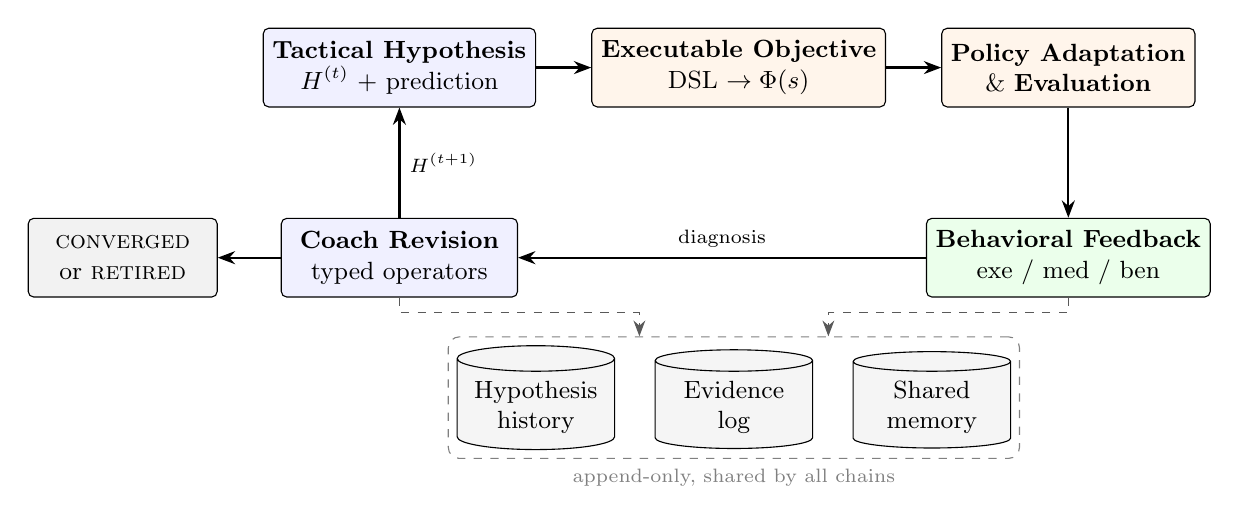
\begin{tikzpicture}[
  node distance=6mm and 7mm,
  box/.style={draw, rounded corners=2pt, align=center, minimum width=30mm, minimum height=10mm, font=\small, fill=#1},
  box/.default=white,
  store/.style={draw, cylinder, shape border rotate=90, aspect=0.18, minimum width=20mm, minimum height=11mm, align=center, font=\small, fill=gray!8},
  arr/.style={-{Stealth[length=2.2mm]}, thick},
  darr/.style={-{Stealth[length=2mm]}, dashed, gray!70!black}
]
\node[box=blue!6]  (hyp) {\textbf{Tactical Hypothesis}\\ $H^{(t)}$ + prediction};
\node[box=orange!8, right=of hyp] (obj) {\textbf{Executable Objective}\\ DSL $\to \Phi(s)$};
\node[box=orange!8, right=of obj] (pol) {\textbf{Policy Adaptation}\\ \& \textbf{Evaluation}};
\node[box=green!8, below=14mm of pol] (fb) {\textbf{Behavioral Feedback}\\ exe / med / ben};
\node[box=blue!6, below=14mm of hyp] (rev) {\textbf{Coach Revision}\\ typed operators};
\node[box=gray!10, left=8mm of rev, minimum width=24mm] (exit) {\textsc{converged}\\ or \textsc{retired}};

\draw[arr] (hyp) -- (obj);
\draw[arr] (obj) -- (pol);
\draw[arr] (pol) -- (fb);
\draw[arr] (fb) -- node[above, font=\scriptsize]{diagnosis} (rev);
\draw[arr] (rev) -- node[right, font=\scriptsize]{$H^{(t+1)}$} (hyp);
\draw[arr] (rev) -- (exit);

\node[store] (E) at ($(rev)!0.5!(fb)+(0,-19mm)$) {Evidence\\ log};
\node[store, left=5mm of E] (H) {Hypothesis\\ history};
\node[store, right=5mm of E] (M) {Shared\\ memory};
\node[draw, dashed, gray, rounded corners, fit=(H)(E)(M), inner sep=3pt, label={[font=\scriptsize, gray]below:append-only, shared by all chains}] (S) {};
\draw[darr] (rev.south) |- ($(S.north)+(-12mm,3mm)$) -- ($(S.north)+(-12mm,0)$);
\draw[darr] (fb.south) |- ($(S.north)+(12mm,3mm)$) -- ($(S.north)+(12mm,0)$);
\end{tikzpicture}
\caption{The refinement loop run by every hypothesis chain. GPU cost is incurred only in policy adaptation; all other steps are LLM calls or programs. All state lives in three append-only stores.}
\label{fig:loop}
\end{figure}

\Cref{fig:loop} shows the loop.
Each step has a fixed input, a fixed output, and a fixed store it writes to; we describe them in order.

% ---------------------------------------------------------------------
\subsection{State: Stores and Frozen Artifacts}
\label{sec:stores}

Three append-only stores carry all state across rounds.
\begin{itemize}[leftmargin=*,itemsep=2pt]
  \item \textbf{Hypothesis history} $\Hst$ holds every version of every hypothesis.
    Each entry points to its \code{parent}, so a chain is a path through $\Hst$, and the diff between adjacent versions is the revision record.
    No separate belief base or revision log is kept.
  \item \textbf{Evidence log} $\Est$ holds one evidence record per training run, linking an objective specification to its measured outcome and diagnosis.
  \item \textbf{Shared memory} $\Mst$ starts empty and accumulates knowledge that belongs to no single hypothesis: procedural lessons (a metric that cannot be compiled, a condition that never fires) and regularities about the environment that recur across tactics.
    It is the only channel through which one chain informs another.
    Unlike $\Hst$ and $\Est$, $\Mst$ records what is \emph{currently believed} rather than what happened; its entries are induced from noisy evidence and may be wrong, so an entry can be superseded by a later one.
    Superseded entries remain for audit but are excluded from prompts.
\end{itemize}

Two artifacts are fixed for an entire campaign.
The \emph{environment specification} \code{env\_spec} declares what the environment supports (offside, goalkeeper, out-of-bounds, penalty area, players per side, \dots); it is a property of the environment and is stated once rather than per hypothesis.
The \emph{metric registry} $\reg$ is the compiler's vocabulary: each metric $m$ that can be computed, the \code{env\_spec} capability it depends on, and its empirical distribution under rollouts of the base policy.
Metrics are written in advance; the LLM selects and parameterizes them but never writes code for a new one.

\paragraph{Reproducibility by replay.}
Both artifacts, including the rollout statistics measured once against $\pi_0$ before the campaign, are versioned and frozen.
Consequently, the \emph{input} of every Coach call is fully determined by the seeds of round 0, the ordered store logs and the Coach configuration.
This is testable: replaying the pipeline must yield prompts identical byte for byte.
The Coach is decoded at temperature 0, so its outputs, and with them the violation feedback of rejected revisions (\cref{sec:revision}), are also repeatable, up to nondeterminism in the inference backend.
Replay is what allows any ablation that changes only the Coach to be rerun on existing evidence without new training.

% ---------------------------------------------------------------------
\subsection{Tactical Hypothesis and Prediction Commitment}
\label{sec:hypothesis}

At the start of each round, the Coach reads every version and every evidence record of the chain, together with the active entries of the shared memory $\Mst$, and writes a new \code{HypothesisEntry} to $\Hst$.

Seeds of round 0 are specified in advance, with \code{parent} set to null; every later version is derived by the Coach from the tail of the chain.
\Cref{tab:fields} lists the fields of an entry and when each is filled; the schema is given in \cref{app:schemas}.
The lifecycle of an entry is read off \code{evidence\_ref} (null means not yet trained) rather than a separate status field, which removes one field that could contradict the others.

\begin{table}[t]
\centering\small
\caption{Fields of a \code{HypothesisEntry} and the step that fills each.}
\label{tab:fields}
\begin{tabularx}{\linewidth}{@{}l l X@{}}
\toprule
Field & Filled by & Meaning \\
\midrule
\code{hypothesis\_id} & Coach & identifier of this version \\
\code{parent} & Coach & previous version; null for a seed of round 0 \\
$C$ & Coach & condition under which the tactic applies, in coach language \\
$A$ & Coach & action our team should take, in coach language \\
$M$ & Coach & mechanism explaining why the tactic should work, in coach language \\
\code{O.execution} & Coach & measurable form of $A$ \\
\code{O.mediator} & Coach & measurable form of $M$ \\
\code{prediction} & Coach, before training & direction (\pUp/\pFlat/\pDown) of three quantities, with confidence and rationale; frozen once written \\
\code{screening} & \cref{sec:adapt} & \code{baseline\_execution} measured on $\pi_0$ \\
\code{evidence\_ref} & \cref{sec:feedback} & the evidence record of this version \\
\code{terminal} & \cref{sec:control}, chain tail only & \textsc{converged} or \textsc{retired} \\
\code{note} & Coach, optional & a semantic caveat the compiler cannot detect \\
\bottomrule
\end{tabularx}
\end{table}

\paragraph{Boundary probing.}
The condition $C^{(t)}$ delimits a range of applicability.
Under a budget of tens of runs, the most informative experiment lies on the \emph{boundary} of that range: one scenario in which $C$ barely holds and one in which it barely fails, testing whether the mechanism actually switches with the condition.
The aim is not to discriminate between competing hypotheses but to locate the boundary of a single one.
Because the gate is soft (\cref{sec:compile}), boundary scenarios can be defined directly in gate space: with $g_C$ the compiled gate, a probe pair consists of sets of initial states
\begin{equation}
  \Xi^{+} = \{ s : g_C(s) \in [\tfrac12, \tfrac12+\delta] \}, \qquad
  \Xi^{-} = \{ s : g_C(s) \in [\tfrac12-\delta, \tfrac12) \},
\end{equation}
sampled from rollouts of the base policy.
Whether this is realizable depends on whether the simulator accepts custom initial states; otherwise probing degrades to post hoc stratification of rollouts from full matches by gate value, with lower statistical power.
\todo{confirm whether MARLadona allows custom initial states.}

\paragraph{Prediction commitment.}
Before any GPU time is spent, the Coach commits a directional prediction $p_q \in \{\pUp, \pFlat, \pDown\}$ with a rationale for each of three quantities $q$:
\begin{center}\small
\begin{tabularx}{0.92\linewidth}{@{}l X X@{}}
\toprule
Quantity $q$ & Meaning & A wrong prediction indicates \\
\midrule
execution & whether our side actually does $A$ & a misjudgment of RL learnability (engineering layer) \\
mediator & whether the opponent responds as $M$ claims & a misjudgment of the mechanism (hypothesis layer) \\
benefit & whether the task-level metric improves & a misjudgment of tactical value (hypothesis layer) \\
\bottomrule
\end{tabularx}
\end{center}
Predictions are written into the entry and frozen, so they cannot be rationalized after the fact.
Compared against outcomes, they yield for each chain the prediction accuracy curve that serves as our primary metric.

\paragraph{The role of $M$.}
$M$ is the field that the mediator directly tests and that the \code{revise\_mechanism} operator acts on.
It belongs to its chain and evolves with it (narrowing $C$ usually forces a matching change in $M$), and it is never lifted into $\Mst$ on its own.
A mechanistic finding is promoted to $\Mst$ only once the same anomaly has appeared on at least two chains, at which point it no longer belongs to any single hypothesis.
We write $M$ as an explicit causal chain (e.g.\ \emph{pressing intensity $\uparrow$ $\to$ opponent errors in back passes $\uparrow$ $\to$ high turnovers $\uparrow$}), whose intermediate quantity is what $O^{\mathrm{med}}$ measures, so that a failure can be localized to a specific link without the cost of a full structural causal model.

The output format is enforced by constrained decoding against the entry schema.

% ---------------------------------------------------------------------
\subsection{Executable Objective}
\label{sec:compile}

The compiler takes the condition $C$ and the observables $O$ of an entry, together with \code{env\_spec} and the metric registry $\reg$, and produces an objective specification $\omega$.
The specification consists of a condition and a potential and nothing else, and it is all that the trainer receives.

\paragraph{Grammar.}
The entire output space of the compiler is the following grammar, which compiles directly into the output schema so that anything outside it is unreachable under constrained decoding:
\begin{align}
  m &\in \reg = \{\textit{team\_width},\ \textit{ball\_x},\ \textit{time\_since\_turnover},\ \dots\}, \\
  \text{gate} &:= \sigma(m,\ \theta,\ w) \in [0,1], \\
  \text{condition} &:= \text{gate} \;\mid\; \text{condition} \wedge \text{condition} \;\mid\; \neg\,\text{condition}, \\
  \text{potential} &:= \textstyle\sum_i w_i \cdot \operatorname{soft}(m_i,\ \ell_i,\ h_i).
\end{align}
All thresholds $\theta, \ell_i, h_i$ and widths $w$ are expressed as \emph{percentiles} of the registry's statistics under the base policy, never as absolute numbers.
Disjunction is not offered as a first-class operator: narrowing adds a conjunct or tightens a percentile, and widening does the reverse.

\paragraph{Soft gate.}
Let $F_m$ be the frozen empirical CDF of metric $m$ under $\pi_0$, and $q_m(s) = 100\,F_m\bigl(m(s)\bigr)$ its percentile rank.
A gate is a sigmoid centered at $\theta$ whose 10--90\% transition spans $w$ percentile points,
\begin{equation}
  \sigma(m, \theta, w)(s) = \frac{1}{1+\exp\!\bigl(-\kappa\,(q_m(s)-\theta)/w\bigr)}, \qquad \kappa = 2\ln 9,
\end{equation}
with conjunction as the product and negation as $1-g$.
The soft potential term is $\operatorname{soft}(m,\ell,h)(s)=\operatorname{clip}\bigl((q_m(s)-\ell)/(h-\ell),\,0,\,1\bigr)$, and weights satisfy $w_i\ge 0$, $\sum_i w_i=1$, so the potential lies in $[0,1]$.
The compiled gate $g_C(s)$ and potential $\psi(s)$ combine into
\begin{equation}
  \Phi(s) = g_C(s)\,\psi(s).
\end{equation}
Softening keeps $\Phi$ continuous, prevents the shaping signal from switching on and off as a metric oscillates around its threshold, and leaves a weak gradient outside the condition, so the policy can learn to \emph{create} the condition rather than only act once it holds.

\paragraph{What is compiled and what is not.}
Only $C$ and $O^{\mathrm{exe}}$ are compiled: $C$ becomes the gate and $O^{\mathrm{exe}}$ becomes the potential.
$A$ and $M$ are claims in coach language and are not passed to the compiler; $A$ is kept, although nearly synonymous with $O^{\mathrm{exe}}$, because it is the form a coach recognizes and the form the chain refines.
$O^{\mathrm{med}}$ is \emph{measured only}.
This is deliberate: a rewarded mediator could be reached by routes that bypass $A$, in which case the ``mechanism refuted'' outcome of \cref{sec:feedback} could never fire.

\paragraph{Reward shaping.}
The shaping reward follows PBRS \citep{ng1999policy},
\begin{equation}
  F(s,s') = \lambda\,\bigl(\gamma\,\Phi(s') - \Phi(s)\bigr), \qquad \tilde r = r + F,
  \label{eq:pbrs}
\end{equation}
with $\Phi(s_{\mathrm{terminal}}) = 0$.
The global magnitude $\lambda$ is not part of the hypothesis.
A badly chosen $\lambda$ can manufacture three different diagnoses (if it is too large, the policy follows the tactic while losing; if it is too small, execution never moves), so we normalize it against the magnitude of task return measured on rollouts of the base policy at a fixed ratio $\rho$ shared by all hypotheses, $\lambda = \rho\,\bar R_0$.
\todo{fix $\rho$ from the study of the base policy.}

\paragraph{Interpretation under PBRS.}
Every metric in $\Phi$ is computed by the simulator from the global state $s$, although no single agent observes all of its inputs.
When $\Phi$ is a function of $s$, the shaping terms of \cref{eq:pbrs} telescope along every trajectory to $-\lambda\,\Phi(s_0)$, which does not depend on the policy; the ranking of joint policies, and hence the set of optimal ones, is therefore unchanged \citep{ng1999policy}, also when policies condition only on local observations.
The effect of a tactic is therefore an \emph{inductive bias under a finite adaptation budget}: it changes which solution an adaptation of $\pi_0$ with a limited budget reaches, not what is optimal in the limit.
We accordingly measure benefit at a fixed adaptation budget and read a hypothesis as a claim about that regime.
Three caveats follow.
Metrics that depend on history, such as \textit{time\_since\_turnover}, are not tracked by MARLadona and must be added to the simulator state; otherwise $\Phi$ is not a function of $s$ and invariance no longer holds.
Partial observability does not affect invariance, but it can make the shaping signal harder to learn from, because an agent may be rewarded for changes in quantities it cannot observe.
And alternatives that alter the action space, such as action masks, change the optimal policy set directly and would require a different reading of the evidence; they are not used in this version.

\paragraph{Registry enforcement and coverage gaps.}
Enforcement has two layers, and only the second is a guarantee.
The registry and \code{env\_spec} enter the system prompt and the available metric names become an \code{enum} in the output schema, so an invented metric is unreachable at decoding time; every metric used is then checked programmatically against \code{env\_spec}, and compilation fails immediately rather than wasting a training run.
A hypothesis that needs a metric the registry lacks fails to compile; the failure is written to $\Mst$ as a procedural entry, and the accumulated list drives the next registry version.
Some semantic degradations remain undetectable by the compiler and are recorded in the optional \code{note} field.
For instance, a tactic of running in behind the last defender compiles and trains successfully in an environment without offside, but its conclusion is meaningless.

\paragraph{Caching.}
The canonical serialization of $\omega$ (canonical JSON, fixed numeric precision) is hashed into a cache key.
Online cache hits are rare, but offline ablations that replay the Coach on existing evidence hit constantly, which is what makes them free.
A cache hit still requires a prediction commitment and produces a new evidence record marked \code{cached\_from}.

% ---------------------------------------------------------------------
\subsection{Policy Adaptation and Evaluation}
\label{sec:adapt}

This step adapts the base policy $\pi_0$ to the objective $\omega$ against the fixed opponent pool $\opp$.
Besides the adapted policy $\pi_\theta$, its training curves and its evaluation metrics, it records \code{baseline\_execution}, the mean gate value and the KL divergence from the base policy.

The step fine-tunes $\pi_0$ with MAPPO \citep{yu2022mappo} on $\tilde r$.
Fine-tuning a converged RL policy as mere weight initialization is fragile: the critic is mismatched to the new return, the policy's entropy has collapsed so the new behavior is rarely sampled, plasticity has decreased, and basic skills (ball control, passing, positioning) may be overwritten so that a drop in performance can no longer be attributed to the tactic.
Following \citet{wolczyk2024finetuning}, we regard adaptation as a problem of mitigating forgetting and add terms for knowledge retention,
\begin{equation}
\begin{split}
  \mathcal{L}(\theta) = \mathcal{L}_{\mathrm{MAPPO}}(\theta)
  &+ \beta_{\mathrm{KS}}\, \E_{s\sim d^{\pi_\theta}}\!\bigl[\KL\bigl(\pi_0(\cdot\mid s)\,\|\,\pi_\theta(\cdot\mid s)\bigr)\bigr] \\
  &+ \beta_{\mathrm{BC}}\, \E_{s\sim \mathcal{D}_0}\!\bigl[\KL\bigl(\pi_0(\cdot\mid s)\,\|\,\pi_\theta(\cdot\mid s)\bigr)\bigr],
\end{split}
\end{equation}
where the first regularizer is kickstarting on on-policy states \citep{schmitt2018kickstarting} and the second is behavioral cloning replay on a fixed buffer $\mathcal{D}_0$ of states visited by the base policy.
The two address different causes of forgetting (states the current policy still visits versus states it no longer reaches); which to use is decided empirically before the campaign and then fixed.

\paragraph{Baseline execution first.}
Before adaptation, $\pi_0$ is run against $\opp$ and its value on the $O^{\mathrm{exe}}$ metric is recorded as \code{baseline\_execution}.
Execution is always reported as a delta from this value; otherwise any tendency the base policy already has would count as the tactic's effect, and hypotheses aligned with that tendency would pass for free.

\paragraph{Diagnostics.}
Two quantities are logged for every run:
\begin{equation}
  \gbar = \E_{s\sim d^{\pi_\theta}}\bigl[g_C(s)\bigr], \qquad
  \mathrm{KL}_0 = \E_{s\sim d^{\pi_\theta}}\bigl[\KL\bigl(\pi_\theta(\cdot\mid s)\,\|\,\pi_0(\cdot\mid s)\bigr)\bigr].
\end{equation}
$\gbar$ indicates whether the shaping signal was generated at all; $\mathrm{KL}_0$ indicates whether the policy moved.
Together they separate ``learned something, but not the intended thing'' from ``did not move'' (\cref{sec:feedback}).

\paragraph{Execution rules.}
\begin{itemize}[leftmargin=*,itemsep=2pt]
  \item \textbf{Paired design.} Every condition starts from the same $\pi_0$ and the same seed set.
    Much of the seed variance in MARL comes from early divergence, and a shared base policy removes that part, so 2--3 seeds suffice; statistical tests must be paired accordingly.
  \item \textbf{Fixed opponent pool, no self-play.} A coevolving opponent slows convergence and makes rounds incomparable, since an improved win rate might only reflect a weaker opponent.
    Comparability across rounds is the premise of the refinement mechanism.
  \item \textbf{Tiered budget.} A screening tier uses one fifth of the step budget and one seed, looking only at the execution trend and the early slope of benefit; a confirmation tier uses the full budget and multiple seeds.
  \item \textbf{Reduced scenarios} for screening (e.g.\ a 3v3 situation in the attacking third), with full matches reserved for confirmation, contingent on simulator support.
\end{itemize}

% ---------------------------------------------------------------------
\subsection{Behavioral Feedback and Outcome Attribution}
\label{sec:feedback}

This step turns the raw output of \cref{sec:adapt} into one \code{EvidenceRecord}, which is written to $\Est$.

Three quantities are computed, all relative to the base policy on matched evaluation:
\begin{align}
  \Delta_{\mathrm{exe}} &= \E\bigl[o^{\mathrm{exe}}(\pi_\theta)\bigr] - \texttt{baseline\_execution}, \\
  \Delta_{\mathrm{med}} &= \E\bigl[o^{\mathrm{med}}(\pi_\theta)\bigr] - \E\bigl[o^{\mathrm{med}}(\pi_0)\bigr], \\
  \Delta_{\mathrm{ben}} &= \mathrm{WR}(\pi_\theta) - \mathrm{WR}(\pi_0),
\end{align}
where $o^{\mathrm{exe}}$ and $o^{\mathrm{med}}$ are the registry metrics named by $O$, and $\mathrm{WR}$ is the win rate against $\opp$, a single task-level definition shared by all hypotheses so that benefit is comparable across them.
Each delta is mapped to an observed direction $o_q \in \{\pUp,\pFlat,\pDown\}$ by a paired significance test, with $\pFlat$ whenever the test does not reject.
The specific test and significance level are fixed in the configuration before the campaign.

\paragraph{Diagnosis.}
The diagnosis is assigned programmatically by the ordered rules of \cref{tab:diagnosis}.
The central idea is that a hypothesis can fail for four reasons: the tactic is wrong, its translation is wrong, RL did not adapt within budget, or the result reflects seed noise.
Only the first may change a belief.
Execution therefore gates everything: if our side did not do what the tactic asks, the run says nothing about the tactic.

\begin{table}[t]
\centering\small
\caption{Programmatic diagnosis. Rules are applied top to bottom; ``$\neg\pUp$'' means \pFlat\ or \pDown. Only the first three rows are evidence about the hypothesis; the rest concern the environment or the pipeline and are routed to the shared memory as candidate entries.}
\label{tab:diagnosis}
\begin{tabularx}{\linewidth}{@{}c c c c l X@{}}
\toprule
& exe & med & ben & Diagnosis & Routed to \\
\midrule
0 & \multicolumn{3}{c}{seeds disagree / not converged} & \code{inconclusive} & shared memory \\
\midrule
1 & \pUp & \pUp & \pUp & \code{belief\_supported} & chain \\
2 & \pUp & \pUp & $\neg\pUp$ & \code{belief\_disconfirmed} (value) & chain; the only case counting toward retirement \\
3 & \pUp & $\neg\pUp$ & any & \code{belief\_disconfirmed} (mechanism) & chain; prefer \code{revise\_mechanism} \\
\midrule
4 & $\neg\pUp$ & -- & -- & \code{condition\_too\_rare} \ ($\gbar < \epsilon_g$) & shared memory; widen $C$ \\
5 & $\neg\pUp$ & -- & -- & \code{insufficient\_adaptation} \ ($\mathrm{KL}_0 < \epsilon_{\mathrm{KL}}$) & shared memory; fix adaptation \\
6 & $\neg\pUp$ & -- & -- & \code{translation\_failure} \ (otherwise) & shared memory; fix compilation \\
\bottomrule
\end{tabularx}
\end{table}

The three rows with flat execution are distinguished by \emph{cause}, not by outcome, because each calls for a different repair: a gate that never opened needs a wider condition, a policy that never moved needs different adaptation hyperparameters, and a policy that moved in the wrong direction needs a different compilation.
Collapsing them would let engineering noise masquerade as belief evidence.
Row 3 captures a distinct and informative case: our team executed the tactic, but the opponent did not respond as $M$ claims.
Even if benefit rose, the stated reason is wrong.

% ---------------------------------------------------------------------
\subsection{Coach Revision}
\label{sec:revision}

After each training run, the Coach reads all versions and evidence of the chain and the active entries of $\Mst$, and returns a sequence of typed revision operators and, optionally, one memory entry.

The Coach is a stateless function of the stores. Revision proceeds in three steps.

\paragraph{1. Induction.}
The discrepancy between the frozen predictions $(p_q)$ and the observed directions $(o_q)$ is distilled into a qualitative revision rule stating \emph{what} must change, not how to realize the change structurally.

\paragraph{2. Revision with typed operators.}
The rule is realized by operators from a closed set (\cref{tab:ops}), applied to the chain tail to derive the next version, which is written to $\Hst$ with \code{parent} pointing to the current tail.
\code{narrow\_condition} is the core operator: in this framework, becoming more accurate mostly means narrowing $C$ to its true range.
With only a handful of evidence records, discarding a whole hypothesis after one failure is overfitting, so smaller edits are preferred.

\begin{table}[t]
\centering\small
\caption{The seven revision operators. All but the last act on a hypothesis chain.}
\label{tab:ops}
\begin{tabularx}{\linewidth}{@{}l X@{}}
\toprule
Operator & Effect \\
\midrule
\code{adjust\_confidence} & change only the confidence of the current version \\
\code{narrow\_condition} & add a conjunct or tighten a percentile in $C$ (core operator) \\
\code{widen\_condition} & remove a conjunct or relax a percentile in $C$ \\
\code{revise\_mechanism} & replace one link of the causal chain $M$ (and the corresponding $O^{\mathrm{med}}$) \\
\code{split} & fork the chain into two versions with complementary, narrower conditions, when evidence shows opposite behavior in different regions \\
\code{retire} & declare the hypothesis wrong; chain terminates \\
\code{retract\_memory} & supersede a shared memory entry contradicted by later evidence \\
\bottomrule
\end{tabularx}
\end{table}

\paragraph{3. Deductive validation by evidence replay.}
The revised hypothesis must still explain \emph{all} historical evidence on its chain.
If it resolves the latest contradiction but conflicts with an earlier record, the revision is rejected and reissued.
Because the Coach runs at temperature 0, reissuing the same prompt would return the same revision; the Coach is therefore called again with the violations $\nu$ of the rejected attempt appended to its input, that is, the identifiers of the evidence records the revision fails to explain and the reference checks below that it fails.
This is pure LLM inference at zero GPU cost, and it directly prevents the Coach from being dragged around by a single noisy round, which is the main failure mode of naive iterative prompting under noisy feedback.

\paragraph{Output constraints.}
Two layers constrain the output.
First, constrained decoding masks tokens that would violate the schema before sampling, so format errors cannot occur; in particular the operator name is a closed \code{enum}.
Structure is constrained tightly (enums, required fields, nesting) while content in natural language (\code{reason}) is left free, since overly strict schemas push the model onto paths of low probability.
Second, programmatic \emph{reference checks} verify what decoding cannot: \code{hypothesis\_id} and \code{trigger\_evidence} must exist, a \code{narrow\_condition} must yield a different non-empty condition, and multiple \code{split} or \code{retire} operations in a single revision are flagged.
Deductive validation is a semantic judgment and stays with the LLM.
The failure rate of reference checks is itself a quantitative measure of model capability and is logged for comparisons across LLM backends.

\paragraph{Memory writes.}
The four diagnoses in \cref{tab:diagnosis} that are not about belief are \emph{candidates} for $\Mst$, not automatic entries.
The threshold depends on the strength of the evidence, not on the diagnosis category: a fact that is self-evident from a single case (a metric that fails to compile, a condition that never fires) may be written after one occurrence, while anything inferred from outcomes (seed variance, effect sizes) requires the same anomaly on at least two chains.
This rule keeps $\Mst$ from becoming a dumping ground, which matters because every active entry enters every prompt.

% ---------------------------------------------------------------------
\subsection{Loop Control}
\label{sec:control}

At the end of each round a chain takes one of three exits:
\begin{itemize}[leftmargin=*,itemsep=2pt]
  \item \textbf{Next version} (default): $H^{(t+1)}$ is written to $\Hst$ and the chain returns to \cref{sec:hypothesis}.
  \item \textbf{Converged}: $k_{\mathrm{conv}}$ consecutive rounds in which all three predictions are correct and no revision beyond \code{adjust\_confidence} is required.
    The output is a rule whose condition has been narrowed to its true range.
    This is the main positive product of the system, not merely ``a hypothesis not yet refuted''.
  \item \textbf{Retired}: $k_{\mathrm{ret}}$ cumulative value disconfirmations (row 2 of \cref{tab:diagnosis}).
    The output is a hypothesis the evidence has judged wrong.
\end{itemize}
$k_{\mathrm{conv}}$ and $k_{\mathrm{ret}}$ are fixed in the configuration before experiments begin and are not adjusted afterwards.
Because seed hypotheses are drawn from soccer practice, we expect refinement to be the common outcome and retirement the rare one; a campaign in which \code{retire} never fires is therefore not evidence of failure, provided \code{narrow\_condition} produces substantive narrowing.

The complete procedure for one chain is summarized in \cref{alg:loop}.
A version that fails to compile is revised in place before any prediction is committed, so the round counter advances only after a training run and every $H^{(t)}$ with $t \ge 1$ has exactly one evidence record $e^{(t)}$ behind it.
Both terminal checks depend on the operators returned by the Coach: convergence requires that they contain nothing beyond \code{adjust\_confidence}, and the confidence update is kept as the final version of the chain.
When the chain is retired, the candidate $H'$ is not used.

\begin{algorithm}[t]
\caption{Refinement of one hypothesis chain}
\label{alg:loop}
\small
\KwData{stores $\Hst,\Est,\Mst$; \code{env\_spec}; metric registry $\reg$;\\
  base policy $\pi_0$; opponent pool $\opp$; training seeds $Z$}
\KwIn{seed hypothesis $H^{(0)}$; thresholds $k_{\mathrm{conv}}, k_{\mathrm{ret}}$}
\KwOut{chain $H^{(0:t)}$ whose tail is marked \textsc{converged} or \textsc{retired}}
$t \leftarrow 0$\;
\While{chain not terminal}{
  \While{$\textsc{Compile}(H^{(t)}.C, H^{(t)}.O^{\mathrm{exe}}, \code{env\_spec}, \reg)$ fails}{
    write procedural entry to $\Mst$\;
    $(\text{ops}, \cdot) \leftarrow \Gamma(H^{(0:t)}, e^{(1:t)}, \Mst, \varnothing)$; $H^{(t)} \leftarrow \textsc{Apply}(\text{ops}, H^{(t)})$\;
  }
  $\omega \leftarrow \textsc{Compile}(H^{(t)}.C, H^{(t)}.O^{\mathrm{exe}}, \code{env\_spec}, \reg)$\;
  $H^{(t)}.\text{prediction} \leftarrow \textsc{CommitPrediction}(H^{(0:t)}, e^{(1:t)}, \Mst)$; append $H^{(t)}$ to $\Hst$\;
  $b \leftarrow \textsc{BaselineExecution}(\pi_0, \omega, \opp)$\;
  $(\pi_\theta, \gbar, \mathrm{KL}_0, \text{metrics}) \leftarrow \textsc{Adapt}(\pi_0, \Phi_\omega, \opp, Z)$\;
  $e^{(t+1)} \leftarrow \textsc{Attribute}(\text{metrics}, b, \gbar, \mathrm{KL}_0)$; append $e^{(t+1)}$ to $\Est$\;
  $\nu \leftarrow \varnothing$\;
  \Repeat{$\nu = \varnothing$}{
    $(\text{ops}, \mu^{(t+1)}) \leftarrow \Gamma(H^{(0:t)}, e^{(1:t+1)}, \Mst, \nu)$\;
    $H' \leftarrow \textsc{Apply}(\text{ops}, H^{(t)})$\;
    $\nu \leftarrow \textsc{ReplayViolations}(H', e^{(1:t+1)}) \cup \textsc{RefCheckViolations}(\text{ops})$\;
  }
  \lIf{$\mu^{(t+1)} \neq \varnothing$}{append $\mu^{(t+1)}$ to $\Mst$}
  \uIf{converged under $k_{\mathrm{conv}}$ given ops}{$H^{(t+1)} \leftarrow H'$; $t \leftarrow t+1$; mark $H^{(t)}$ \textsc{converged}; append $H^{(t)}$ to $\Hst$\;}
  \uElseIf{retired under $k_{\mathrm{ret}}$ \textbf{or} \code{retire} $\in$ ops}{mark $H^{(t)}$ \textsc{retired}\;}
  \lElse{$H^{(t+1)} \leftarrow H'$; $t \leftarrow t+1$}
}
\end{algorithm}

% =====================================================================
\section{Iteration Efficiency}
\label{sec:efficiency}

A naive implementation (training from scratch, one hypothesis per round, three or more seeds) supports only five to ten rounds, too few for the ablations of \cref{sec:protocol}.
We combine the following levers.
Policy adaptation from a shared base policy avoids relearning locomotion, passing and positioning, and its paired design reduces the required seeds.
Running four chains in parallel with two seeds each keeps wall-clock time constant while quadrupling information.
Tiered screening discards most poor candidates in the first fifth of the budget, and reduced scenarios may cut the cost of screening by a further order of magnitude if the simulator supports custom player counts and initial states.
Our conservative estimate is 15--25 rounds with four hypotheses per round.
These figures are extrapolated from general MARL experience and remain to be measured on MARLadona.

Parallelism interacts with the shared memory.
Chains advanced later inherit a larger memory and should converge faster, while chains advanced in parallel cannot see each other's results within a round.
We therefore fix the execution order before the campaign, report each chain's index, and include it as a covariate in the analysis; once order is controlled for, a positive effect of chain index can be reported as evidence that the memory carries useful knowledge rather than as a confound.

% =====================================================================
\section{Evaluation Protocol}
\label{sec:protocol}

\subsection{Environment, Base Policy and Seed Hypotheses}

We use MARLadona \citep{li2025marladona} on Isaac Lab with its continuous command action space.
A base policy is trained by self-play until competent, then frozen.
\code{env\_spec} is written from a survey of the environment's action and observation spaces, rules (offside, out-of-bounds, goalkeeper, penalty area, set pieces) and configurability.
The metric registry contains 10--15 metrics with frozen percentile statistics under $\pi_0$.

The first batch consists of twelve seed hypotheses drawn from common soccer principles (\cref{tab:seeds}).
Each seed starts an independent chain.
Their original descriptions were edited in two ways: observables that merely restate the action (e.g.\ ``team width increases'' for a widening tactic) were moved to $O^{\mathrm{exe}}$, since they only show that the shaping took effect, and statements of benefit were removed, since benefit is measured by a common task-level metric.

\begin{table}[t]
\centering\footnotesize
\caption{Seed hypotheses of round 0 (condition and action abbreviated). The last column marks seeds whose condition refers to an opponent trait rather than a field state; these cannot fire unless the opponent pool contains that trait.}
\label{tab:seeds}
\begin{tabularx}{\linewidth}{@{}l X X l@{}}
\toprule
ID & Condition $C$ & Action $A$ & Opp.\ trait \\
\midrule
H-001 & opponent compact centrally & widen our positional structure & \\
H-002 & opponents concentrated on ball side & switch play quickly to the weak side & \\
H-003 & channel opens between opponent lines & play forward immediately & \\
H-004 & opponent defensive line high & runs in behind the last defender$^{\dagger}$ & high line \\
H-005 & ball concentrated on one side & attacker on far side attacks back post & \\
H-006 & opponent attempts central progression & compress spacing between our players & \\
H-007 & center more dangerous than flanks & block central lanes, induce play wide$^{\ddagger}$ & \\
H-008 & opponent builds up short from the back & coordinated high press & short build-up \\
H-009 & possession just lost, players near ball & immediate counter-press & \\
H-010 & first counter-press broken & stop chasing, recover centrally & fast counter \\
H-011 & possession just won, opponent disorganized & progress forward on first touches & \\
H-012 & ball won but opponent counter-presses & exit pressure zone / find player on far side & counter-press \\
\bottomrule
\end{tabularx}\\[2pt]
\raggedright\scriptsize $^{\dagger}$Without an offside rule this degenerates into goal-hanging. $^{\ddagger}$The mediator is nearly mechanical; the substantive claim is at the benefit level.
\end{table}

\paragraph{Opponent pool (open).}
A frozen copy of $\pi_0$ satisfies the requirement of a fixed pool, but a single opponent makes a third of the seeds untestable and leaves converged conditions open to the objection that they encode one opponent's fingerprint rather than the tactic's boundary.
Training checkpoints are a cheap but poor source of diversity, since early and late checkpoints differ in strength rather than behavioral trait.
We instead plan to build trait variants with the same compiler used for hypotheses (e.g.\ training an opponent under a ``hold a high defensive line'' potential), so that traits are defined rather than labeled after the fact and pool coverage can be checked programmatically.
A minimal pool is $\pi_0$ plus three compiled variants (high line, counter-press, short build-up).
Open questions include the number of variants, whether traits acquired in training fire conditions often enough to learn from, and whether opponents are sampled uniformly or matched to each hypothesis.
The pool composition will be reported with every converged hypothesis.

\subsection{Metrics}
\label{sec:metrics}

\paragraph{Prediction accuracy per chain (primary, zero GPU cost).}
For round $t$ of a chain,
\begin{equation}
  \mathrm{acc}_t = \frac{1}{3}\sum_{q\in\{\mathrm{exe},\mathrm{med},\mathrm{ben}\}} \mathbb{1}\bigl[p_q^{(t)} = o_q^{(t)}\bigr].
\end{equation}
We report the curve per chain rather than as an aggregate: a chain whose accuracy rises over rounds is direct evidence that \emph{this} hypothesis has become more accurate.
The metric does not depend on task performance or RL luck and can be recomputed for any Coach configuration on the same evidence.

\paragraph{Condition specificity (zero GPU cost).}
The trigger rate $\tau(C) = \E_{s\sim d^{\pi_0}}[g_C(s)]$ under frozen rollouts of the base policy measures how far $C$ has been narrowed.
A healthy chain shows decreasing $\tau(C)$ while the effect inside the condition remains significant.

\paragraph{Operator usage and failures of reference checks.}
Operator frequencies diagnose the quality of refinement: rising accuracy dominated by \code{narrow\_condition} indicates healthy condition refinement, whereas flat accuracy with no \code{retire} and mostly \code{adjust\_confidence} indicates that the Coach is rationalizing rather than learning.
Failure rates of reference checks are compared across LLM backends.

\paragraph{Guarding against excessive narrowing.}
Narrowing taken to the extreme overfits: a condition shrunk to exactly the scenarios that happened to be tested shows a strong effect that does not generalize.
Three defenses apply: the preference for minimal edits, deductive validation against all earlier evidence, and one confirmation run per converged chain on scenarios that did not participate in its refinement.

\subsection{Ablations}

\Cref{tab:ablations} lists the ablations.
Most require no new training because the stores permit replay.

\begin{table}[t]
\centering\small
\caption{Ablations and the question each answers.}
\label{tab:ablations}
\begin{tabularx}{\linewidth}{@{}l X X l@{}}
\toprule
Condition & Setting & Question & New training \\
\midrule
Full & chains + predictions + deductive validation & -- & yes \\
Random feedback & execution/benefit labels shuffled across rounds, marginals preserved & Does the Coach use the evidence or only soccer priors? & no \\
Raw evidence ICL & evidence stacked in context, no chain structure & What does the chain add over plain in-context learning? & partial \\
No chain & each round starts afresh from the last result only & Is this just iterative prompting? & partial \\
Frozen hypothesis & no revision after round 1 & Is refinement across rounds necessary? & partial \\
No deduction & evidence replay removed & What is deductive validation worth? & no \\
Order shuffle & evidence order permuted, fold rerun & Is path dependence refinement or a random walk? & no \\
Chain index & fixed order, index as covariate & Does memory, or tactic simplicity, speed later chains? & no \\
Matched tokens & equal reasoning budget across conditions & Do gains come only from longer context? & no \\
\bottomrule
\end{tabularx}
\end{table}

\paragraph{Random feedback as the key test.}
Prior work on lab-in-the-loop agents reports that falsified feedback can hurt more than no feedback \citep{labloop2026}.
If our Coach's accuracy degrades under shuffled labels, it is demonstrably using the evidence.
The test is free because it replays existing records.

\paragraph{LLM backends.}
Model capability is a genuine confound: a negative result from one model cannot distinguish a flawed method from an insufficiently capable model.
The main experiments are therefore run with both an open-weight model (Qwen3.8-27B, Apache-2.0, served with INT4 quantization) and a commercial API, with constrained decoding on both (xgrammar locally, structured outputs for the API) so that format adherence is removed as a variable and only content quality differs.
Pipeline debugging uses a smaller local model.
Commercial calls are pinned to dated model identifiers at temperature 0, and every prompt and response is archived.

\subsection{Results}
\todo{Pending.
Planned: (i) prediction accuracy curves per chain for the twelve seeds; (ii) trajectories of trigger rate with effect sizes inside the condition; (iii) histograms of operator usage; (iv) replays with random feedback and without deduction; (v) growth of the shared memory over rounds; (vi) diagnosis distribution, in particular the share of diagnoses that are not about belief.}

% =====================================================================
\section{Discussion and Limitations}
\label{sec:discussion}

\paragraph{Marginal gains from structure.}
In clean, high-throughput settings, explicit belief structures have yielded only modest improvements over stacking evidence in context \citep{labloop2026}.
Our argument for a larger benefit here is that with one noisy result per round, a hypothesis derived again from scratch is easily swayed by the latest outcome, whereas a chain with deductive validation integrates evidence across rounds.
This argument must be confirmed by the raw evidence ICL ablation rather than assumed.

\paragraph{Shaping magnitude and PBRS semantics.}
Benefit is measured at a fixed adaptation budget and so reflects the tactic as an inductive bias rather than a change of the optimum.
Conclusions are conditional on the adaptation budget, the retention regularizers and the shaping ratio $\rho$; all are fixed before the campaign and reported.

\paragraph{Opponent dependence.}
A converged condition is a statement about the environment \emph{and} the opponent pool.
Without trait diversity it may encode one opponent's weaknesses.
Pool composition is therefore part of every reported result.

\paragraph{Prior knowledge.}
LLMs have read extensive soccer literature, which may inflate zero-shot baselines.
In our formulation this is a lesser concern: literature supplies the prior and the simulator supplies evidence specific to the environment, and disagreement between the two is exactly what the system is designed to resolve.

\paragraph{Environment fidelity.}
Simplified simulators lack rules (e.g.\ offside) or behaviors that some tactics presuppose.
The compiler catches missing capabilities; silent semantic degradations are only flagged through hypothesis notes and remain a risk.

% =====================================================================
\section{Conclusion}
\label{sec:conclusion}

We presented Coach LLM, a framework in which an LLM refines tactical hypotheses, rather than policies or rewards, from the behavioral evidence of MARL training.
Its central design choices follow from the cost and noise of that evidence: hypotheses are structured to be falsifiable, outcomes are decomposed so that only genuine tactical evidence can change a belief, revisions are typed, minimal and validated against all earlier evidence, and all state is kept in append-only stores so that the Coach can be studied offline at no training cost.
The next step is to close the loop on MARLadona and test whether hypothesis chains measurably become more accurate.

\clearpage
\bibliographystyle{plainnat}
\bibliography{refs}

% =====================================================================
\clearpage
\appendix

\section{Schemas}
\label{app:schemas}

\paragraph{HypothesisEntry.}
\begin{lstlisting}[style=json]
{
  "hypothesis_id": "H-007",
  "C": "...", "A": "...", "M": "...",
  "O": { "execution": "...", "mediator": "..." },
  "parent": "H-003",
  "prediction": { "execution": "up", "mediator": "up", "benefit": "up",
                  "confidence": "Medium", "rationale": "..." },
  "screening": { "baseline_execution": 0.31 },
  "evidence_ref": "R3",
  "terminal": null,
  "note": null
}
\end{lstlisting}

\paragraph{EvidenceRecord.}
\begin{lstlisting}[style=json]
{
  "evidence_id": "R3", "round_id": 3, "hypothesis_id": "H-007",
  "objective_spec": { "condition": "...", "potential": "..." },
  "objective_hash": "sha256:...", "cached_from": null,
  "outcome": {
    "execution": { "delta_vs_baseline": 0.41, "significant": true },
    "mediator":  { "delta_vs_baseline": 0.05, "significant": false },
    "benefit":   { "winrate_delta_vs_base": 0.02, "significant": false },
    "kl_from_base": 0.18, "mean_gate": 0.27,
    "base_policy_id": "P-base-v2", "opponent_pool_id": "OP-fixed-01",
    "seeds": [0, 1], "paired": true
  },
  "diagnosis": "belief_disconfirmed",
  "training_meta": { "sim": "MARLadona", "algo": "MAPPO", "commit": "..." }
}
\end{lstlisting}
Numbers are illustrative of the format only.

\paragraph{RevisionOp.}
\begin{lstlisting}[style=json]
class RevisionOp(BaseModel):
    op: Literal["adjust_confidence", "narrow_condition", "widen_condition",
                "revise_mechanism", "retire", "split", "retract_memory"]
    hypothesis_id: str
    trigger_evidence: str
    reason: str
\end{lstlisting}

\paragraph{MemoryEntry.}
\begin{lstlisting}[style=json]
{
  "memory_id": "M-003",
  "content": "Conditions gated on the goalkeeper having the ball trigger in under 2% of timesteps; avoid them when designing conditions.",
  "trigger_diagnosis": "condition_too_rare",
  "trigger_evidence": ["R7", "R11"],
  "status": "active", "superseded_by": null, "created_round": 4
}
\end{lstlisting}

\end{document}
